\documentclass[a4paper]{article}
\usepackage[a4paper,margin=3mm]{geometry}

% default stuff
\usepackage{amsmath}
\usepackage{amssymb}
\usepackage{enumitem}

% multicolumn package
\usepackage{multicol}

\usepackage{multirow}
\usepackage{makecell}
\renewcommand\theadfont{\bfseries}

\newcolumntype{M}[1]{>{\centering\arraybackslash} m{#1}} % centered m

\newcommand{\abs}[1]{\left\lvert#1\right\rvert}

\newcommand{\ol}[1]{\begin{enumerate}#1\end{enumerate}}
\newcommand{\oll}[1]{\begin{enumerate}[leftmargin=*]#1\end{enumerate}}
\newcommand{\ul}[1]{\begin{itemize}#1\end{itemize}}
\newcommand{\ull}[1]{\begin{itemize}[leftmargin=*]#1\end{itemize}} % no margin

% coloring code
\usepackage{color}
\definecolor{dkgreen}{rgb}{0,0.6,0}
\definecolor{gray}{rgb}{0.5,0.5,0.5}
\definecolor{mauve}{rgb}{0.58,0,0.82}

\definecolor{lg}{rgb}{0.9,0.9,0.9}

% code environment
\usepackage{listings}
\lstset{
  %frame=tb, % adds top and bottom border
  aboveskip=1mm,
  belowskip=1mm,
  showstringspaces=false,
  columns=flexible,
  basicstyle={\small\ttfamily},
  numberstyle=\color{gray},
  keywordstyle=\color{blue}\textbf,
  commentstyle=\color{dkgreen},
  stringstyle=\color{mauve},
  breaklines=true,
  breakatwhitespace=true,
  tabsize=4
}
\newcommand{\ic}[1]{\lstinline{#1}}

% drawing a stack diagram
\usepackage{drawstack}
\usetikzlibrary{arrows.meta}

\newcommand{\ptr}[1]{${}^{*}$#1}
\newcommand{\addr}[1]{\&#1}
\newcommand{\addrb}[1]{(\&#1)}

% special table column for code
\usepackage{collcell}
\newcommand*{\tablecode}[1]{\lstinline{#1}}% Do anything you like with `#1`
\newcolumntype{T}{>{\collectcell\tablecode}c<{\endcollectcell}}


\graphicspath{ {./images/} }

% \@startsection{<name>}{<level>}{<indent>}{<beforeskip>}{<afterskip>}{<style>}*[<altheading>]{<heading>}
% \titlespacing*{\section}      {0pt}{3.5ex plus 1ex minus .2ex}{2.3ex plus .2ex}
% \titlespacing*{\subsection}   {0pt}{3.25ex plus 1ex minus .2ex}{1.5ex plus .2ex}
% \titlespacing*{\subsubsection}{0pt}{3.25ex plus 1ex minus .2ex}{1.5ex plus .2ex}
% \titlespacing*{\paragraph}   {0pt}{3.25ex plus 1ex minus .2ex}{1em}

% reduce spacing before and after headers
\makeatletter
\renewcommand{\section}{
  \@startsection{section}{1}{0pt}{1ex}{1.5ex}{\normalfont\large\bfseries}}
\renewcommand{\subsection}{
  \@startsection{subsection}{2}{0pt}{1ex}{1ex}{\normalfont\normalsize\bfseries}}
% 5th arg is different for paragraph
\renewcommand{\paragraph}{
  \@startsection{paragraph}{4}{0pt}{1.5ex}{-0.8em}{\normalfont\bfseries}}

% line separating cols
\setlength{\columnseprule}{0.3pt}

% remove page numbering
\pagenumbering{gobble}

% math-mode version of "c" column type
\newcolumntype{C}{>{$}c<{$}}

% TODO:
% - time complexity, stability, invariants of sorts (L6 S79)
% - T6

\begin{document}
\footnotesize

% First page
\begin{multicols}{3}
  \lstset{language=Java, backgroundcolor=\color{lg}}
  \part*{\centering \underline{CS2040S}}
  \section*{\underline{Java}}
    \ull {
      \item Use \ic{Object.equals(Object o)} to compare objects
      \item String concatenation takes $O(\text{length})$
    }
  \section*{\underline{Big-O notation}}
    \paragraph{Upper bound} $T(n) = O(f(n))$ if for some $c > 0$ and $n_0 > 0$,
      \[ T(n) \leq c f(n) \]
      for all $n > n_0$.
    \paragraph{Lower bound} $T(n) = \Omega(f(n))$ if for some $c > 0$ and $n_0 > 0$,
      \[ T(n) \geq c f(n) \]
      for all $n > n_0$.
    \paragraph{Tight bound} $T(n) = \Theta(f(n))$ if
      \[ T(n) = O(f(n)) \quad\text{and}\quad T(n) = \Omega(f(n)) \]
    \paragraph{Properties}
      Let $T(n) = O(f(n))$ and $S(n) = O(g(n))$.
      \oll {
        \item If $T(n)$ is a polynomial of degree $k$ then
          \[ T(n) = O(n^k) \]
        \item Addition: $T(n) + S(n) = O(f(n) + g(n))$
        \item Multiplication: $T(n) \times S(n) = O(f(n) \times g(n))$
        \item Max: $\max(T(n), S(n)) = O(f(n) + g(n))$
        \item Composition: $T(S(n)) = O(f \circ g(n))$ only if both functions are increasing
      }
    \paragraph{Overview}
      \begin{align*}
        1 < \log n < \sqrt{n} < n < n \log n \\ < n^2 < n^3 < 2^n < 2^{2n} < n! < n^n
      \end{align*}
    \paragraph{Stirling's approximation}
      $ n! \approx \sqrt{2 \pi n} \left(\dfrac{n}{e}\right)^n $ \\
      Used to show that $\log(n!) = O(n \log n)$
    \paragraph{Geometric series}
      \[ S_n = a + ar + ar^2 + \cdot + ar^{n-1} = \frac{a(1-r^n)}{1-r} \]
    \paragraph{Harmonic series}
      $ \sum_{i=1}^\infty \frac{1}{i} = O(\log n) $
    \paragraph{Logarithm change of base}
      $ \log_b a = \dfrac{\log_x b}{\log_x a} $
    \paragraph{Master theorem} Comparing $f(n)$ with $n^{\log_b(a)}$ as polynomials, for $a \geq 1$ and $b > 1$,
      \[
        \begin{aligned}
          & T(n) \\
          &= a T\left( \frac{n}{b} \right) + f(n) \\
          &= \begin{cases}
               \Theta(n^{\log_b(a)}) & \text{if } f(n) < n^{\log_b(a)} \\
               \Theta(n^{\log_b(a)} \log n) & \text{if } f(n) = n^{\log_b(a)} \\
               \Theta(f(n)) & \text{if } f(n) > n^{\log_b(a)} \\
             \end{cases}
        \end{aligned}
      \]
  \section*{\underline{Algorithms}} \noindent
    (with binary search as example algo)
    \paragraph{Precondition} Fact that is true before algorithm runs.
      e.g. Array is sorted
    \paragraph{Postcondition} Fact that is true when algorithm ends.
      e.g. If element in array, then \ic{A[begin] = key}
    \paragraph{Invariant} Relationship between variables that is always true
    \paragraph{Loop invariant} Invariant at beginning/end of loop
      e.g. \ic{A[begin] <= key <= A[end]}, i.e. key is in range
    \subsection*{Peak finding}
      Assume \ic{A[-1]} and \ic{A[n]} are \ic{-INT_MAX}.
      \begin{lstlisting}
FindPeak(A, n)
  mid = n/2
  if A[mid+1] > A[mid] then recurse on right half
  elif A[mid-1] > A[mid] then recurse on left half
  else A[mid] is a peak
      \end{lstlisting}
      If we recurse into right half, then:
      \ul {
        \item Given that \ic{A[mid] < A[mid+1]} (condition for recursing into right half)
        \item Assuming no peak, then \ic{A[mid] < A[mid+1] < A[mid+2] < ... < A[n-1] > A[n] = -INT_MAX}
        \item Hence peak must exist
      }
  \section*{\underline{Sorting}}
    \paragraph{Bubble} compare adjacent and swap to make right $>$ left
    \paragraph{Selection} find smallest element and swap it to end of sorted region
    \paragraph{Insertion} swap each new element until it is correctly placed within sorted region
    \paragraph{Small arrays} Insertion sort is stable, works fast for nearly sorted arrays, has little overhead.
    \paragraph{Merge} (recursive) sort each half and merge
    \paragraph{Quicksort} (recursive) partition about a pivot
    \paragraph{In-place partitioning} $O(n)$
      \oll {
        \item Choose a random pivot (for good quicksort performance), and swap it to the start
        \item Increase \ic{lptr} while element at left $<$ pivot
        \item Decrease \ic{rptr} while element at right $>$ pivot
        \item If not yet at centre, swap pointers and repeat
      }
    \paragraph{Quicksort variations}
      \ull {
        \item Is stable only if the partitioning is stable. Requires $O(n)$ extra space to store initial indices
        \item If pivot splits by a fraction, good enough
        \item 3-way partitioning: pack duplicates in middle to eliminate duplicate elements worst case
        \item Paranoid: force a good pivot
        \item $k$-pivots: $O(k \log k)$ to sort pivots + $O(n \log k)$ to binary search the pivots to choose correct bucket to place the new item. $T(n) = O(n \log_k n \log k) = O(n \log n)$, i.e. no performance improvements
        \item 2-pivot quicksort is in practice better than 1-pivot quicksort, because of cache performance
      }
    \paragraph{Quickselect} Like quicksort, but only recurse on relevant half of partitioned array
    \subsection*{Probability}
      \paragraph{Linearity of expectation} For random variables $X$ and $Y$:
        \[ E(aX + bY) = a E(X) + b E(Y) \]
        \paragraph{Expected trials} If an event $X$ has probability of success $p$, then an expected $\tfrac{1}{p}$ trials is required for 1 success.
    \subsection*{Order Statistics}
      \paragraph{Find $k$th smallest element} Quicksort but only recurse on relevant side - $O(n)$
    \subsection*{Interval Tree} \noindent
      Each node stores an interval, keyed on left endpoint, augmented with max right endpoint in subtree
      \paragraph{Search} $O(\log n)$
        \oll {
          \item If value in node interval, return node
          \item If \ic{value > node.left.max}, recurse right
          \item Else recurse left
        }
        \paragraph{All-overlaps} If we want to find all $k$ intervals that contain value - $O(k \log n)$
        \oll {
          \item Search for interval
          \item Add to list and delete interval
        }
    \subsection*{Orthogonal Range Searching}
      \ull {
        \item Leaf nodes contain points
        \item Internal nodes contain max in left subtree
        \item Build tree: $O(n \log n)$, Space: $O(n)$
      }
      \paragraph{Search} Find number of points in range $[a, b]$ - $O(k + \log n)$, where $k$ is number of points found
        \oll {
          \item Find split node, highest node with key in range $[a, b]$
          \item Do left child traversal
            \ull {
              \item If node in query range, then add entire right subtree to list, and recurse left
              \item Else recurse right
            }
          \item Do right child traversal (similar)
        }
      \paragraph{n dimensional search}
        \ull {
          \item Recursively store $d-1$ dim range tree in each node of a 1D range tree
          \item Build tree: $O(n \log^{d-1} n)$, Query: $O(\log^d n + k)$
          \item Space: $O(n \log^{d-1} n)$, 2D tree Rotate: $O(n)$
        }
  \section*{\underline{Trees}}
    \subsection*{Binary trees}
      \ull {
        \item A binary tree is either empty, or a node pointing to two binary trees.
        \item In a balanced tree, $h = O(\log n)$
        \item Height is no. of edges on longest path to leaf
      }
      The following operations are all $O(\log n)$:
      \paragraph{searchMin} keep going left
      \paragraph{searchMax} keep going right
      \paragraph{search, insert} go left/right depending on comparison of new key with cur key
      \paragraph{successor}
        \ull {
          \item If node has right child: \ic{right.searchMin()}
          \item Else traverse upwards until ancestor contains node in left subtree, then return ancestor
        }
      \paragraph{predecessor}
        \ull {
          \item If node has left child: \ic{left.searchMax()}
          \item Else traverse upwards until ancestor contains node in right subtree, then return ancestor
        }
      \paragraph{delete}
        \ull {
          \item 0 children: remove node
          \item 1 child: remove node, connect parent to child
          \item 2 children: delete successor (at most 1 child), replace node value with successor value
        }
      The following operations are all $O(n)$:
      \paragraph{in-order} left, self, right
      \paragraph{pre-order} self, left, right
      \paragraph{post-order} left, right, self
      \paragraph{level-order} decreasing height (BFS)
      \paragraph{Ancestor} Node $x$ is an ancestor of node $y \Leftrightarrow x$ comes before $y$ in pre-order, AND $y$ comes before $x$ in post-order.
\end{multicols}

\vspace{-1.7\baselineskip}
\hrulefill
\vspace{-1.0\baselineskip}

% Recurrence time complexity
\begin{multicols}{3}
  % hacky solution to reduce unnecessary vertical spacing
  {\centering
    $O(1)$ work \\ \vspace{.2cm}
    $ \displaystyle
    \begin{aligned}
      T(n) &= T (\tfrac{n}{k}) + O(1) = O(\log n) \\
      T(n) &= kT (\tfrac{n}{k}) + O(1) = O(n) \\
      T(n) &= kT (\tfrac{n}{2k}) + O(1) = O(\sqrt n)
    \end{aligned}
    $
  \par}
  {\centering
    Not $O(1)$ work \\ \vspace{.2cm}
    $ \displaystyle
    \begin{aligned}
      T(n) &= T (\tfrac{n}{k}) + O(n) = O(n) \\
      T(n) &= kT (\tfrac{n}{k}) + O(n) = O(n \log n) \\
      T(n) &= kT (\tfrac{n}{k}) + O(n \log n) = O(n \log^2 n)
    \end{aligned}
    $
  \par}
  {\centering
    Subtract in recurrence \\ \vspace{.2cm}
    $ \displaystyle
      \begin{aligned}
        T(n) &= T(n-c) + O(n) = O(n^2) \\
        T(n) &= 2T(n-1) + O(1) = O(2^n) \\
        T(n) &= T(n-1) + T(n-2) + O(1) = O(\phi^n)
      \end{aligned}
    $
  \par}
\end{multicols}

% Second page
\begin{multicols}{3}
  \subsection*{AVL trees}
    \ull {
      \item A node $v$ is height balanced if \\
        \ic{|v.L.height - v.R.height| <= 1}
      \item A height balanced tree has at $h < 2 \log n$ (actually, approximately $\dfrac{1}{\log \phi} \log n$)
    }
    \paragraph{Balancing}
      Assume A is \underline{left-heavy}. Otherwise, if A is right-heavy, substitute ALL left, right with right, left
      \\\\
      Define B as left child of A.
      \\\\
      Case 1: B is \textbf{balanced:} \ic{rightRotate(A)}
      \begin{center}
        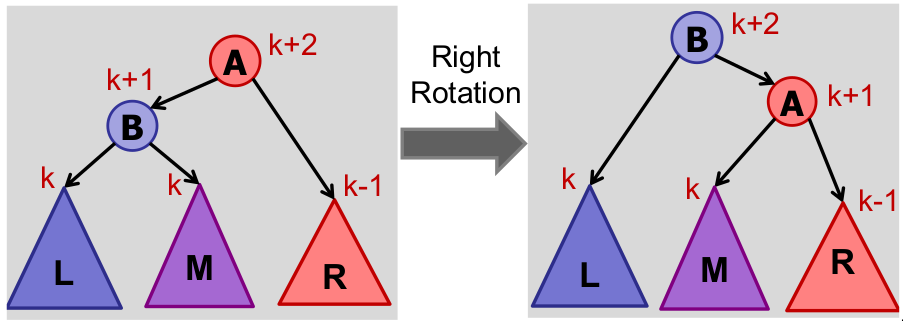
\includegraphics[width=0.28\textwidth]{AVL_Case_1}
      \end{center}
      Case 2: B is \textbf{left-heavy:} \ic{rightRotate(A)}
      \begin{center}
        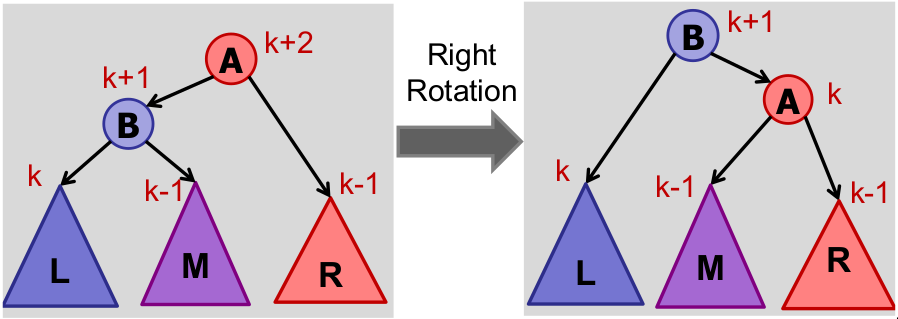
\includegraphics[width=0.28\textwidth]{AVL_Case_2}
      \end{center}
      Case 3: B is \textbf{right-heavy:} \\
        \ic{leftRotate(A.left); rightRotate(A)}
      \begin{center}
        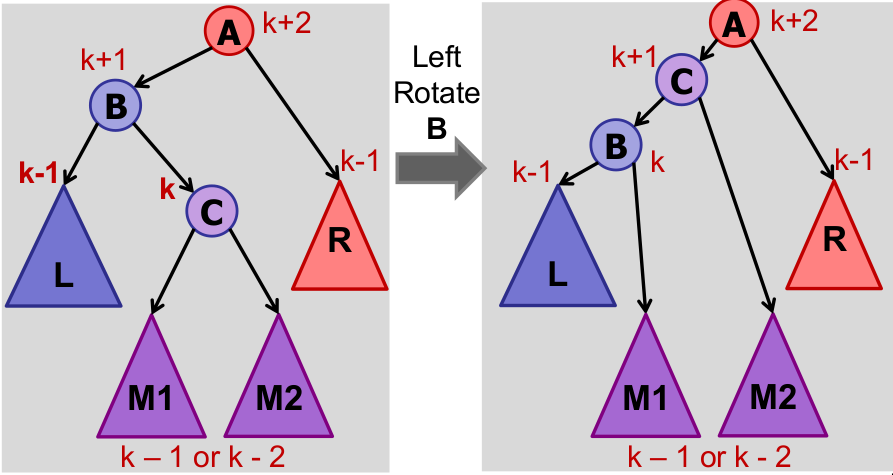
\includegraphics[width=0.28\textwidth]{AVL_Case_3a}
        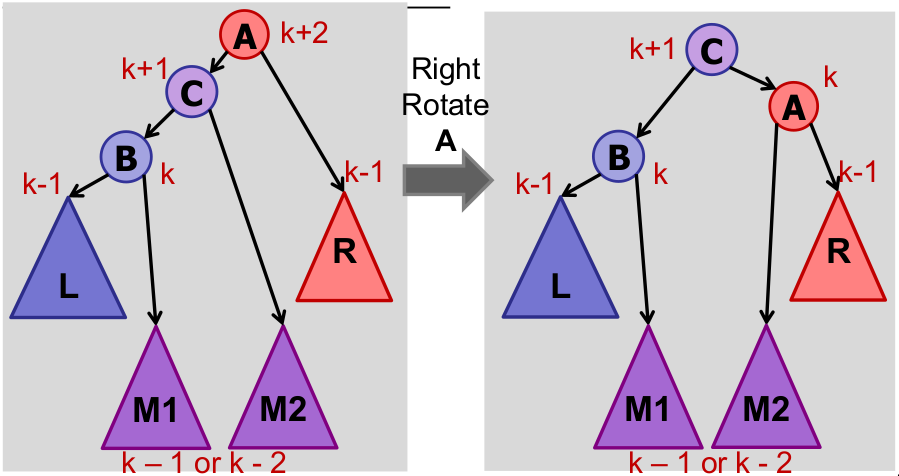
\includegraphics[width=0.28\textwidth]{AVL_Case_3b}
      \end{center}
      Update weights after \ic{rightRotate(A)}
      \begin{center}
        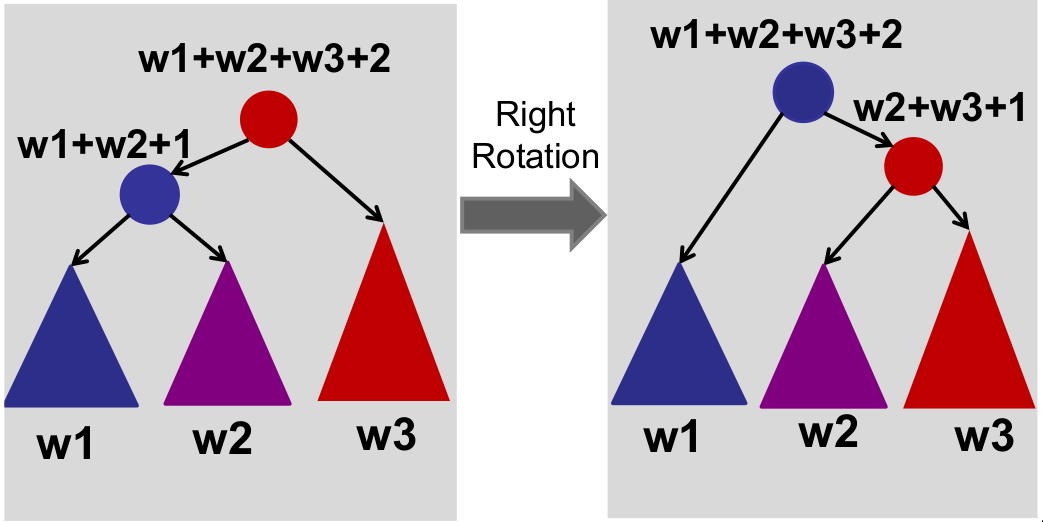
\includegraphics[width=0.28\textwidth]{AVL_weights}
      \end{center}
      Update max after \ic{rightRotate(A)}
      \begin{center}
        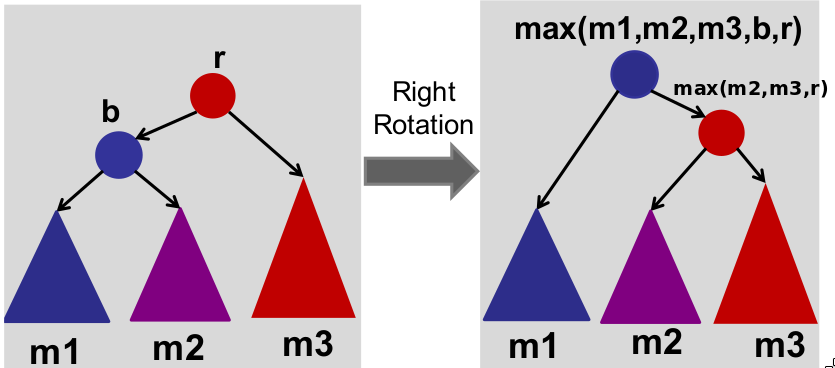
\includegraphics[width=0.28\textwidth]{AVL_max}
      \end{center}
      \ull {
        \item Insertion: max 2 rotations
        \item Deletion: max $O(\log n)$ rotations
      }
    \paragraph{Rank of node} Position in in-order
\begin{lstlisting}
rank(node):
  rank = node.L.weight + 1
  while node != null
    if node is right child
      rank += node.parent.L.weight + 1
    node = node.parent
  return rank
\end{lstlisting}
  \subsection*{Trie}
    \ull {
      \item search, insert: $O(L)$
      \item space: $O\Big(\sum L + \text{overhead}\Big)$
    }
  \subsection*{$k$-d tree}
    \ull {
      \item Stores coordinates in $x-y$ plane
      \item Levels alternate between splitting plane by $x$ or $y$
    }
    \paragraph{Search node} $O(\log n)$
      \oll {
        \item If horizontal split, compare $x$-coordinate
        \item If vertical split, compare $y$-coordinate
        \item $O(h)$ time
      }
    \paragraph{Search min} $O(\sqrt n)$ (e.g. min $x$)
      \oll {
        \item If horizontal split, recurse left child
        \item If vertical split, recurse on both children
        \item $T(n) = 2T(\frac{n}{4}) + O(1)$
      }
    \paragraph{Build} $O(n \log n)$
      \oll {
        \item Choose either $x$ or $y$.
        \item Quickselect median of $x$ or $y$: $O(n)$
        \item Split array into two halves using median \\
          Partioning: $O(n)$
      }
  \subsection*{$(a,b)$-tree}
    \begin{center}
      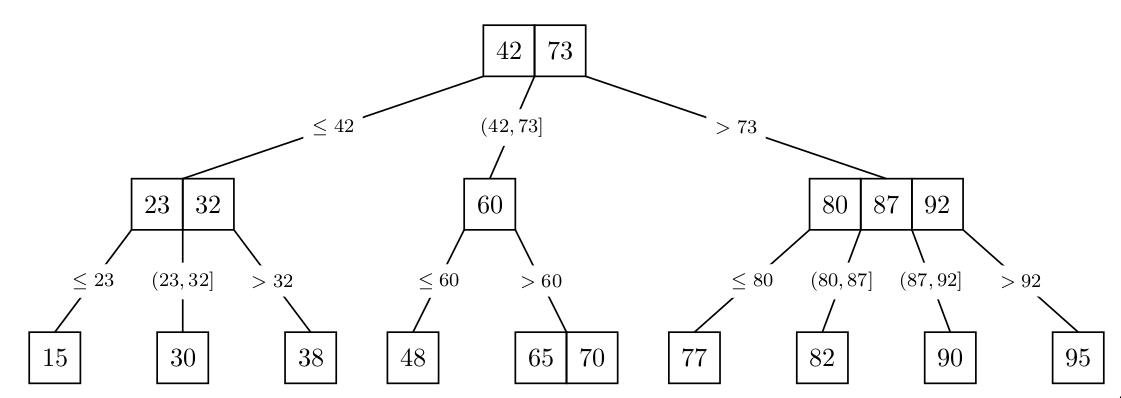
\includegraphics[width=0.28\textwidth]{AB_tree}
      \\
      Sample $(2,4)$-tree
    \end{center}
    \paragraph{Rules}
      \oll {
        \item $(a,b)$ child policy
          \begin{center}
            \begin{tabular}{ |c|c|c|c|c| }
              \hline
              & \multicolumn{2}{c|}{\# Keys} & \multicolumn{2}{c|}{\# Children} \\ \hline
              Node & Min & Max & Min & Max \\ \hline
              Root & 1 & $b-1$ & 2 & $b$ \\ \hline
              Internal & $a-1$ & $b-1$ & $a$ & $b$ \\ \hline
              Leaf & $a-1$ & $b-1$ & 0 & 0 \\ \hline
            \end{tabular}
          \end{center}
        \item A non-leaf node must have one more child than its number of keys
        \item All leaf nodes must all be at the same depth
      }
    \paragraph{Definitions}
      \ull {
        \item Key range: Range of keys allowed in a subtree (wrt parent)
        \item Key list: List of keys in node (assume sorted)
        \item Tree list: List of children
      }
    \paragraph{$B$-tree} simply $(B,2B)$ trees
    \paragraph{Search} $O(\log n)$:
      \ull {
        \item $O(\log b)$ binary search keylist for subtree containing the key to search
        \item Repeat along height of $O(\log_a n)$
      }
    \paragraph{Insert} $O(\log n)$: Like search, then perform split/merge as necessary
      \ull {
        \item Proactive: preemptively split nodes at full capacity (only applies if $b \geq 2a$)
        \item Passive: insert then check (potentially splitting all the way to root)
      }
    \paragraph{Delete} $O(\log n)$: Like search, then perform split/merge as necessary
    \paragraph{Split}
      \begin{center}
        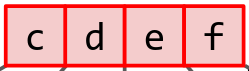
\includegraphics[width=0.14\textwidth]{B-tree/split_before}
        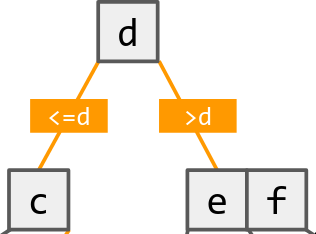
\includegraphics[width=0.14\textwidth]{B-tree/split_after}
      \end{center}
      \oll {
        \item Pick median key of overfull range $z$ as new split key $k$
        \item Put $k$ into parent
        \item Split $z$ into LHS and RHS of $k$
        \item If parent is overfull, \ic{split(parent)}
      }
    \paragraph{Merge}
      \begin{center}
        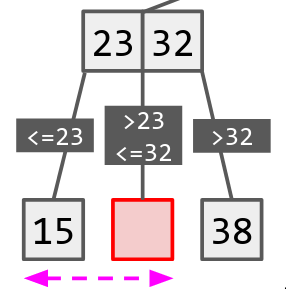
\includegraphics[width=0.14\textwidth]{B-tree/merge_before}
        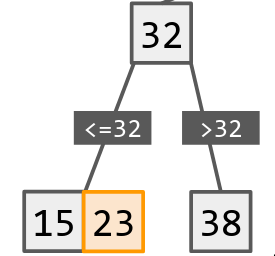
\includegraphics[width=0.14\textwidth]{B-tree/merge_after}
      \end{center}
      Let $d$ be deleted node, and $l$ be left sibling of $d$. Assume keylist of $l$ and $d$ have $< b-1$ keys in total. Otherwise use share below
      \oll {
        \item Pick key $k$ from parent, on left of $d$
        \item Move $k$ to keylist of $l$
        \item Merge $d$ keylist, treelist into $l$
        \item Delete $d$
      }
    \paragraph{Share} \ic{merge(l, d)}; split newly combined node
\section*{\underline{Hashing}}
  \subsection*{Hash functions}
    \ull {
      \item Maps universe to keys in $[1, m]$
      \item Store item with key $k$ in bucket $hash(k)$
      \item Since universe size larger, collisions inevitable by pigeonhole principle
    }
    \paragraph{Simple uniform hash}
      \ull {
        \item Each key has equal probability of being mapped to each bucket
        \item Keys are mapped independently
      }
    \paragraph{Chaining}
      Assume $n$ keys have been inserted into hash table of size $m$.
      \ull {
        \item Each bucket $c$ stores linked list of items with $hash(k) = c$
        \item Insert: $O(1 + hash) = O(1)$
        \item Total space: $O(n + m)$
      }
    \paragraph{Search}
      \ull {
        \item Worst case: $O(n + hash) = O(n)$
        \item Expected case: $O(1 + \frac{n}{m})$, good $m$: O(1)
      }
    \paragraph{Expected max cost of $n$ inserts}
      \ull {
        \item $O(\log n) = \Theta( \frac{\log n}{\log \log n} )$
      }
\end{multicols}

% Sort summary
\begin{center}
  \begin{tabular}{ |c|C|C|C|c|C|c| }
    \hline
    \textbf{Sort} & \textbf{Best} & \textbf{Average} & \textbf{Worst} & \textbf{Stable} & \textbf{Memory} & \textbf{Invariant (after $k$ iterations)} \\ \hline
    Bubble & \Omega(n) & O(n^2) & O(n^2) & \checkmark & O(1) & last $k$ elements in correct final position \\ \hline
    Selection & \Omega(n^2) & O(n^2) & O(n^2) & $\times$ & O(1) & first $k$ elements in correct final position \\ \hline
    Insertion & \Omega(n) & O(n^2) & O(n^2) & \checkmark & O(1) & (original) first $k$ elements in relative sorted order \\ \hline
    Merge & \Omega(n \log n) & O(n \log n) & O(n \log n) & \checkmark & O(n) & subarray is sorted \\ \hline
    Quick & \Omega(n \log n) & O(n \log n) & O(n^2) & $\times$ & O(1) & pivot is in correct final position \\ \hline
  \end{tabular}
\end{center}
\end{document}
